\section{Web Interface}
Es war seit Anfang an klar, dass ein Web-Interface gestaltet werden sollte. Das Web-Interface ist ideal um die Leistung der Software hautnah zu erleben. Man kann mit jedem internetfähigen Gerät (mit Mikrofon) darauf zugreifen.

Die Idee ist einfach. Man nimmt direkt im Browser eine kurze Audioaufnahme auf, lädt diese hoch zum Server, und dieser antwortet mit der geschätzten Sprache. Bevor man die Aufnahme hochlädt kann man sie optional selbst abspielen.
%\\ Aktuell läuft ein Web-Server unter: \url{jo.guru.ksz.ch/deeplid}


\subsection{Frontend}
\begin{figure}[hbt]
	\centering
		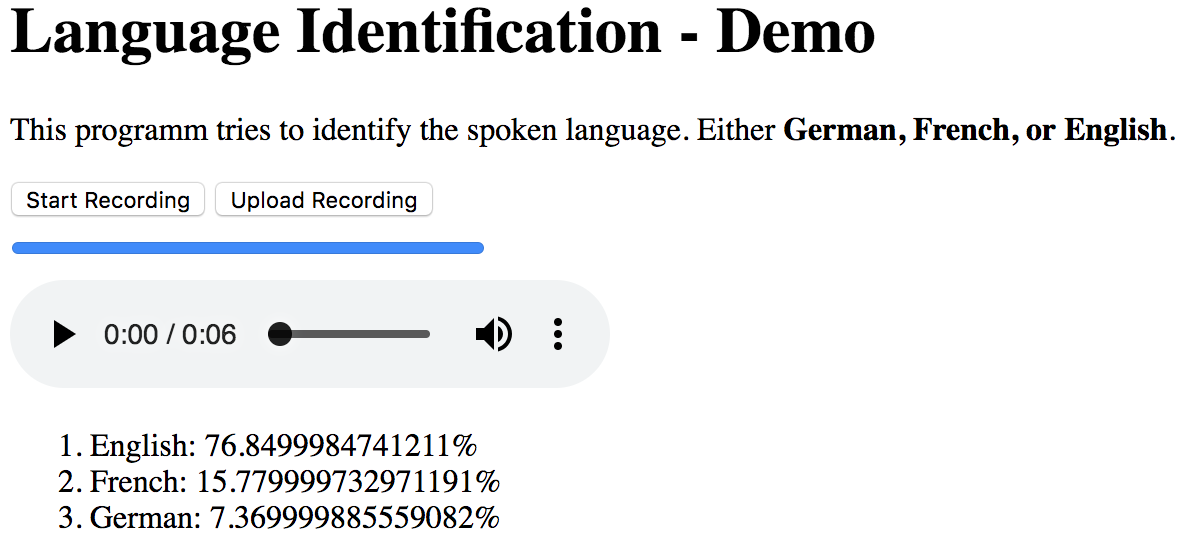
\includegraphics[width=0.6\textwidth]{assets/interface.png}
	\caption{Web-Interface Screenshot}
	\label{img:interface}
\end{figure}
Das Design ist in einfachem \textit{HTML} und \textit{CSS} geschrieben, die Logik mit \textit{Javascript}. Um im Browser Audioaufnahmen nehmen zu können, wird \textit{RecordRTC}\cite{recordrtc} verwendet. \textit{RecordRTC} ist eine unter der \textit{MIT} Lizenz veröffentlichte \textit{Javascript} Bibliothek für Medienaufnahmen. Sie ist kompatibel mit vielen modernen Browsern und Geräten.

Nach der Aufnahme wird die Datei über AJAX POST an den Server verschickt. Der Server antwortet mit einem XML-Snippet der Resultate.
Dieses wird wiederum direkt in die Webseite eingebaut.


\subsection{Backend}
Der Webserver läuft in der Programmiersprache \textit{Python}. Als Framework wird mit \textit{Flask}\cite{flask} verwendet. Da sowohl der \textit{Flask} wie auch \textit{Keras} mit Python laufen, kann der Webserver das trainierte Modell ohne zusätzliche Hürden verwenden.
Der Code findet sich unter \ref{code:webserver}
